\documentclass{article}
%
\usepackage{mathbbol}

\usepackage{ctex}
\usepackage{geometry}
\usepackage[dvipsnames, svgnames, x11names]{xcolor}
\usepackage[mathscr]{euscript}
\usepackage{tikz}
\usepackage{xstring}
%

\usetikzlibrary{decorations.pathreplacing}
\usetikzlibrary{positioning, arrows.meta, automata}
%
%
\begin{document}
%
\begin{center}
  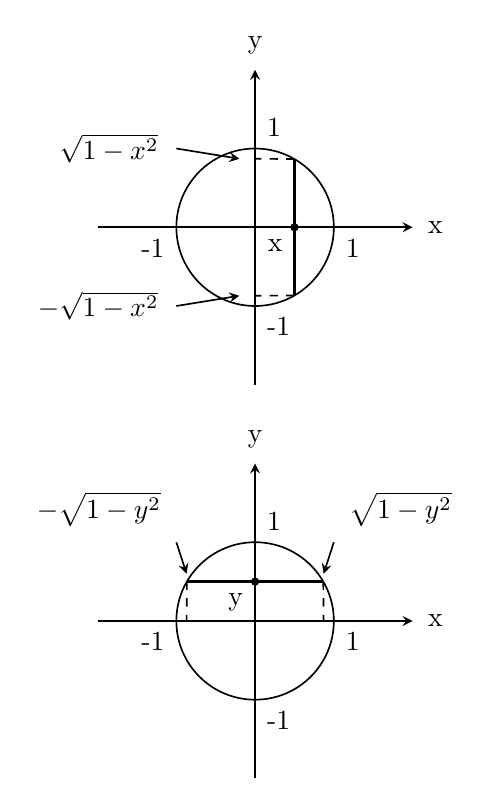
\begin{tikzpicture}[->,>=stealth,node distance=2cm,semithick,initial text=,]

    \draw[->] (-2,0) to (2,0);
    \draw[->] (0,-2) to (0,2);
    \draw[-] (0,2) node [above = 2pt]{y};
    \draw[-] (2,0) node [right = 2pt]{x};

    \draw[-] (1,0) node [below right = 1pt]{1};
    \draw[-] (-1,0) node [below left = 1pt]{-1};
    \draw[-] (0,-1) node [below right = 1pt]{-1};
    \draw[-] (0,1) node [above right = 1pt]{1};
    \draw[-] (0.5,0) node [below left = 1pt]{x};
    \fill (0.5,0) circle (1.5pt);

    \draw[-, very thick] (60:1) to (-60:1);
    \draw[-, dashed] (60:1) to (0,0.87);
    \draw[-, dashed] (-60:1) to (0,-0.87);

    \draw[->] (-1, 1) to (-0.2, 0.87);
    \draw[-] (-1, 1) node [left = 0.1cm]{$\sqrt{1-x^2}$};
    \draw[->] (-1, -1) to (-0.2, -0.87);
    \draw[-] (-1, -1) node [left = 0.1cm]{$-\sqrt{1-x^2}$};
    \draw[-] (0,0) circle (1);

    \tikzset{shift={(0,-5)}};

    \draw[->] (-2,0) to (2,0);
    \draw[->] (0,-2) to (0,2);
    \draw[-] (0,2) node [above = 2pt]{y};
    \draw[-] (2,0) node [right = 2pt]{x};

    \draw[-] (1,0) node [below right = 1pt]{1};
    \draw[-] (-1,0) node [below left = 1pt]{-1};
    \draw[-] (0,-1) node [below right = 1pt]{-1};
    \draw[-] (0,1) node [above right = 1pt]{1};
    \draw[-] (0,0.5) node [below left = 1pt]{y};
    \fill (0,0.5) circle (1.5pt);

    \draw[-, very thick] (150:1) to (30:1);
    \draw[-, dashed] (150:1) to (-0.87,0);
    \draw[-, dashed] (30:1) to (0.87,0);

    \draw[->] (-1, 1) to (-0.87, 0.6);
    \draw[-] (-1, 1) node [above left = 0.1cm]{$-\sqrt{1-y^2}$};
    \draw[->] (1, 1) to (0.87, 0.6);
    \draw[-] (1, 1) node [above right = 0.1cm]{$\sqrt{1-y^2}$};
    \draw[-] (0,0) circle (1);
    


  \end{tikzpicture}
  \heiti\\ 图(a)(b) 关于X的边缘分布与关于Y的边缘分布\songti
\end{center}
%
\end{document}
